Cette partie montre comment mettre en place tous les éléments pour reproduire les attaques évoquées précédemment. On commencera donc par installer ONOS, mininet, puis on téléchargera certains outils pour reproduire les attaques.

\subsection{Installation d'ONOS}

Choisir une machine (virtuelle ou non) sur laquelle installer le contrôleur (durant le stage j'ai utilisé une debian serveur avec accès ssh pour y mettre ONOS). Sur la machine, installer java8 si il ne l'est pas encore. Cloner le dépôt des sources du contrôleur à l'adresse \url{https://gerrit.onosproject.org/onos}. Cloner également le dépôt git à l'adresse \url{https://github.com/Alkanoor/ONOS-Attack.git}. Télécharger apache-karaf et maven.

\begin{minted}{bash}
$ git clone https://gerrit.onosproject.org/onos -b 1.7.0
$ git clone https://github.com/Alkanoor/ONOS-Attack.git
$ mkdir Downloads Applications
$ cd Downloads
$ wget http://archive.apache.org/dist/karaf/3.0.5/apache-karaf-3.0.5.tar.gz
$ wget http://archive.apache.org/dist/maven/maven-3/3.3.9/binaries/apache-maven
 -3.3.9-bin.tar.gz
$ tar -zxvf apache-karaf-3.0.5.tar.gz -C ../Applications/
$ tar -zxvf apache-maven-3.3.9-bin.tar.gz -C ../Applications/
$ cd ..
\end{minted}

\subsection{Installation de Mininet}

Il est possible de suivre les instructions à l'adresse \url{http://mininet.org/download/}. Télécharger l'image qui convient la plus récente sur github (actuellement 2.2.1) : \url{https://github.com/mininet/mininet/wiki/Mininet-VM-Images}. La machine virtuelle offre un accès ssh avec les identifiants \textit{mininet / mininet}.

Il est également possible d'installer mininet sur une machine virtuelle déjà existante en clonant \url{git://github.com/mininet/mininet} et en exécutant \textit{mininet/util/install.sh} dans le dossier mininet.

Sur la machine virtuelle utilisée (si ça n'est pas la même que celle contenant ONOS), cloner également le dépôt \url{https://github.com/Alkanoor/ONOS-Attack.git}

\subsection{Configuration}

Pour que les attaques soient faciles à exécuter, les identifiants par défaut ne seront pas changés. Par contre il faut évidemment que la machine virtuelle contenant ONOS et celle contenant Mininet soient sur un même sous réseau.

Après avoir cloné le dépôt contenant les attaques sur les 2 machines, on va faire un test basique pour vérifier que tout fonctionne. Pour commencer on va configurer rapidement ONOS. Tout d'abord il faut éditer le fichier \textit{org.apache.karaf.features.cfg} en ajoutant mvn:org.onosproject/onos-features/1.7.0-SNAP-SHOT/xml/features (avec une virgule pour séparer le nouvel élément des attributs déjà présents) au niveau des lignes "featuresRepositories" et "featuresBoot" du fichier.

\begin{minted}{bash}
$ nano ~/Applications/apache-karaf-3.0.5/etc/org.apache.karaf.features.cfg
$ #modifier la ligne featuresRepositories en y ajoutant mvn:org.onosproject/onos-
$ #features/1.7.0-SNAPSHOT/xml/features
$ #et la ligne featuresBoot en y ajoutant onos-api,onos-core-trivial,onos-cli,
$ #onos-openflow,onos-app-fwd,onos-gui
\end{minted}

Ensuite, on édite le fichier \textit{onos/tools/dev/bash\_profile} et on le charge dans le .bashrc (cela permet de bien mettre à jour l'environnement). Utiliser maven une première fois pour remplir le fichier profile.

\begin{minted}{bash}
$ echo '#ONOS environment'>>~/.bashrc
$ echo . $(pwd)/onos/tools/dev/bash_profile>>~/.bashrc
$ cd onos
$ ../Applications/apache-maven-3.3.9/bin/mvn clean
\end{minted}

Pour changer les identifiants par défaut (\textit{grep \$(pwd)/onos/tools/dev/bash\_profile -e "ONOS"} changer les variables ONOS\_USER et ONOS\_GROUP avec le nom de l'utilisateur actuel (elles valent normalement "sdn"), et éventuellement les variables ONOS\_WEB\_USER, ONOS\_WEB\_PASS (identifiants pour l'interface web)).
Quitter le shell en cours pour charger le nouveau .bashrc (ou le charger directement avec source).
Puis compiler ONOS (ceci prend un certain temps (au minimum une dizaine de minutes)).

\begin{minted}{bash}
$ mvn clean install
\end{minted}

Lancer ONOS avec
\begin{minted}{bash}
$ ok clean #onos-karaf clean
\end{minted}

Il est possible que toutes les variables nécessaires ne soient pas encore présentes dans l'environnement. Dans ce cas, redémarrer la VM. Si après cela il y a encore des erreurs de programmes non trouvables (onos-karaf, karaf), exporter les variables KARAF\_ROOT et ONOS\_ROOT en cherchant où sont localisés les exécutables.
Pour vérifier que l'installation a fonctionné, on peut accéder à l'URL \url{http://}[adresse du contrôleur sur le réseau]\url{:8181/onos/ui/login.html\#/topo} avec les logins indiqués (si rien n'a été changé, karaf/karaf permet de se connecter à l'interface graphique).

Sur la machine contenant mininet, se placer dans le dossier ONOS-Attack et exécuter le fichier general\_topology.py en lui indiquant l'adresse du contrôleur sur le réseau :
\begin{minted}{bash}
$ sudo python general_topology.py [addresse IP du contrôleur]
\end{minted}

Ensuite activer l'affichage des hôtes sur ONOS et éxecuter la commande \textit{pingall} dans Mininet. Si quelque chose de semblable est obtenu sur l'interface graphique, tout s'est bien déroulé :
\begin{figure}[h]
  	\centering
  	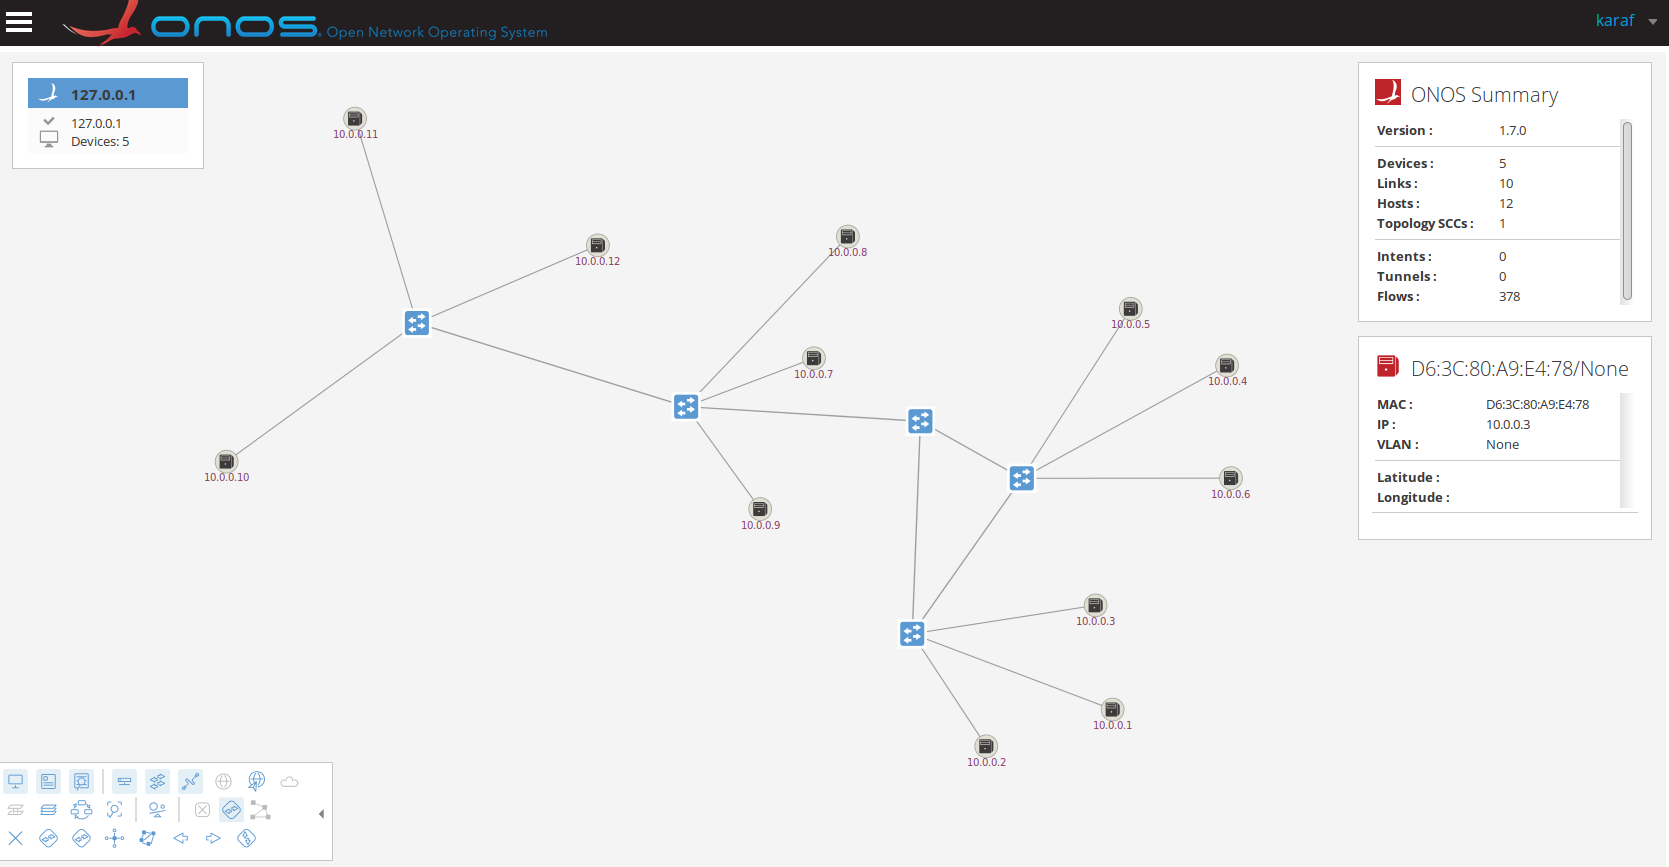
\includegraphics[width=1\textwidth]{onos_GUI.png}
  	\caption{Installation réussie si le résultat est quelque chose de semblable}
\end{figure}